
\chapter{Probability of good eviction choices with sampling\label{sec:sampling-probabilities}}

This appendix analyses the probability of an optimal eviction decision using PBM-sampling. 

This analysis assumes that access time predictions are accurate, or more specifically, that the estimated access order of next access times is accurate. It also assumes sampling with replacement, so that each buffer sampled has the same probability of being optimal independently of the rest of the sample. For single eviction this assumption is actually true -- the PBM-sampling implementation does not check for duplicate samples. For bulk eviction the sampling is also done with replacement, but if the same buffer is sampled multiple times it will only be evicted once, so fewer than the desired number of buffers are evicted. These calculations ignore this possibility, which will happen extremely infrequently since the number of buffers is much larger than the sample size, (and 8~GiB buffer pool of 8 KiB blocks has a million buffers, with sample sizes being on the order of 10-100) so this is a very close approximation.


In general, let $p$ be the probability that any given buffer in the cache is optimal to evict, and has higher next access time than all non-optimal buffers in the cache as discussed in Chapter~\ref{sec:generalized-MIN}. (or equivalently, $p$ is the fraction of the buffers in the cache which are optimal to evict)



\section{Single eviction}

Single eviction selects $N$ samples and evicts the single best one. If any of the $N$ samples are an optimal choice it is chosen for eviction, and a sub-optimal choice requires that none of items in the sample are optimal, so the probability of an optimal eviction is $1-(1-p)^N$, and the long-run expected fraction of optimal evictions is also $1-(1-p)^N$, assuming that $p$ stays constant and each eviction is independent.  % these assumptions probably don't hold in general


\section{Bulk-eviction}

Let $M$ be the number of samples selected and $k$ be the number of evictions. Note that the description in Chapter~\ref{sec:sampling-bulk-eviction} has $M=kN$, but this does not need to be true in general.

Consider the expected number of optimal evictions in one batch of $k$ evictions. This will depend on how many of the $M$ samples are optimal: if it is $<k$ then the number of optimal candidates in the sample is the same as the number of optimal candidates evicted. If there are $\ge k$ optimal candidates in the sample, then only $k$ are evicted. The number of optimal choices from the $M$ samples follows a binomial distribution with $M$ trials and probability of success $p$. Let $P(i) = {M \choose i} p^i (1-p)^{M-i}$ be the probability that $i$ of the $M$ samples are optimal choices.

Then the expected number of optimal evictions from one batch is:
\begin{align*}
    E[\text{\# optimal evictions per batch}] &= \sum_{i=0}^{k-1}{i\cdot P(i)} + \sum_{i=k}^{M}{k\cdot P(i)}\\ 
    &=  \sum_{i=0}^{k-1}{i\cdot P(i)} + k\left( 1-\sum_{i=0}^{k-1}{P(i)} \right)\\
    &= k + \sum_{i=0}^{k-1}(i-k)P(i)\\
    &= k - \sum_{i=0}^{k-1}{(k-i){M \choose i}p^i (1-p)^{M-i}}
\end{align*}
Note than when $M=N$ and $k=1$, this is the same as the result for single eviction.

Since $k$ items are evicted at a time, the proportion of evictions which are optimal is: $1 - \sum_{i=0}^{k-1}{\left(1 - \frac{i}{k}\right) {M \choose i} p^i (1-p)^{M-i}}$

% Formatted for wolframalpha:  k - sum {(k-n) (M choose n) p^n (1-p)^(M-n)}, n=0 to k-1

Figure \ref{plot:P-opt-bulk-eviction} compares the probability of optimal eviction decisions with and without bulk eviction for selected parameters. At a base sample size of 10, grouping 10 evictions together improves the eviction decisions considerably compared to separate independent evictions. The graph shows that evicting 10 of 100 samples is similar to single eviction with a sample size of 20, as also demonstrated by the experiments in Chapter~\ref{sec:eval_sample_size}.



\begin{figure}
    \centering
    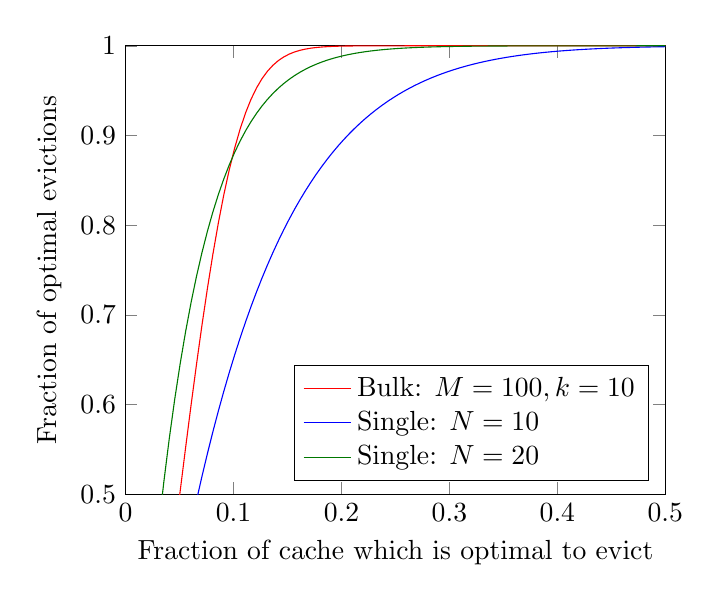
\begin{tikzpicture}
    \definecolor{darkgreen}{RGB}{0,120,0}
    \begin{axis}[
        domain=0:0.5, xmin=0, xmax=0.5,
        range=0.5:1, ymin=0.5, ymax=1,
        samples=100,
        legend pos=south east,
        legend cell align={left},
        xlabel=Fraction of cache which is optimal to evict,
        ylabel=Fraction of optimal evictions,
    ]

    \addplot[color=red]{1 - (1-x)^100 - 90 * x * (1-x)^99 - 3960 * x^2 * (1-x)^98 - 113190 * x^3 * (1-x)^97 - 2352735 * x^4 * (1-x)^96 - 37643760 * x^5 * (1-x)^95 - 476820960 * x^6 * (1-x)^94 - 4802268240 * x^7 * (1-x)^93 - 37217578860 * x^8 * (1-x)^92 - 190223180840 * x^9 * (1-x)^91)};
    % formula expanded with wolframalpha because sums and "choose" function are not available in pgfplot to my knowledge...
    \addlegendentry{Bulk: $M=100, k=10$};
    
    \addplot[color=blue]{1-(1-x)^10};
    \addlegendentry{Single: $N=10$};
    \addplot[color=darkgreen]{1-(1-x)^20};
    \addlegendentry{Single: $N=20$};
    
    \end{axis}
    \end{tikzpicture}
    \caption{Probability of an optimal eviction comparing single- vs bulk-eviction}
    \label{plot:P-opt-bulk-eviction}
\end{figure}